\subsection{Sensor-based Observing Systems Approach to Engineering and Environmental Science}\label{sec:domains}

The use of sensor-based observing systems to both gather data and perform experiments in engineering and environmental science is now a commonly used technique in the efforts to answer questions related to issues such as global warming, invasive species, infectious diseases, structural engineering, desertification, salination, pollution, and land use.  NEON~\cite{NEON}, NEES~\cite{NEES}, GLEON~\cite{GLEON},
CREON~\cite{CREON}, ORION~\cite{ORION}, and EarthScope~\cite{earthscope} are examples of large-scale observatories which are evolving to consist of thousands of sensors, tens of thousands of data streams, and tens of thousands of end users.  Rapid advancements in technology and cyberinfrastructure have made it possible to create and use sensor networks with capabilities that were previously unattainable.  

This paper is based on our experience in providing cyberinfrastructure to a number of observing systems domains and communities.  All of them face similar challenges in deploying and managing a distributed collection of heterogeneous sensors and instruments. Each observatory though has their own unique requirements that mean the individual solutions to these challenges vary greatly from system to system.
We briefly describe some representative domains here, and the interested reader is invited to pursue the references for more information.

The National Ecological Observatory Network (NEON) will be the first national ecological measurement and observation system designed both to answer regional- to continental-scale ecological questions and to have the interdisciplinary participation necessary to achieve credible ecological forecasting and prediction~\cite{NEON}. A key requirement for NEON is robust streaming data middleware to handle thousands of data streams from a large variety of sensing devices. While the NEON sites are distributed, the administration is done through a single central authority.
The Network for Earthquake Engineering and Simulation (NEES) is a shared national network of fifteen experimental facilities, collaborative tools, a centralized data repository~\cite{NEES}. NEES also has a central repository where post-experiment data is uploaded into a data center.  However, individual sites also collaborate on distributed experiments using RBNB DataTurbine to stream data between laboratories.
The Global Lake Ecological Observatory Network (GLEON) is a grassroots network of limnologists, information technology experts, and engineers who have a common goal of building a scalable, persistent network of lake ecology observatories~\cite{GLEON}.  The GLEON sites are geographically distributed and administered locally.  
The Coral Reef Environmental Observatory Network (CREON) is a worldwide collaborative association of scientists and engineers working to design marine sensor networks~\cite{CREON}.  As with GLEON, the CREON sites are also geographically distributed with local administration.  

While no two observatories are identical, there are strong commonalities. For classification purposes, we can divide into two categories based on how control and data are distributed and shared. The first category is federated data model, and the second is the centralized data model. 

\begin{figure*}
\begin{center}
\mbox{
\subfigure[Observing systems: federated model.\label{fig:obsdist}]{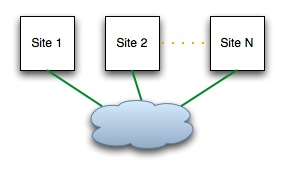
\includegraphics[scale=0.40]{figs/obsdist}} \quad
\subfigure[Observing systems: centralized model.\label{fig:obs-center}]{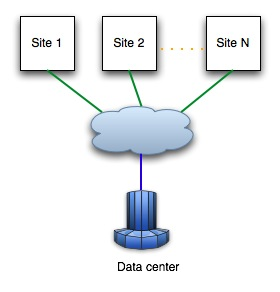
\includegraphics[scale=0.40]{figs/obs-center}}
}
\caption{Observing system models}
\label{fig:obsmodel}
\end{center}
\end{figure*}    

\emph{Federated model:} Participating sites are geographically distributed and are administrated locally (under autonomous control), at the site-level (ref. Figure~\ref{fig:obsdist}). In particular, each site can design its own architecture, database schema and manage its own data using that schema. Thus, the system from sensor to data resource, and the interfaces to the rest of the participating sites (and the world) are the responsibility of the site. 

\emph{Centralized model:} Participating sites are geographically distributed but are administrated by a single administrative authority (ref. Figure~\ref{fig:obsdist}). All the sites gather their data and typically stream/upload it to a data center typically following a common database schema. It is therefore the responsibility of the data center to make the data available for the entire network of participants.

Regardless of their model, all these projects have similar cyberinfrastructure (CI) requirements with regard to data acquisition, instrument management, and state-of-health monitoring including, reliable data capture and transport, persistent monitoring of numerous data channels, automated processing, event detection, analysis, integration across heterogeneous resources and systems, real-time tasking and remote operations and secure access to system resources. To that end, streaming data middleware provides the framework for application development and integration.

\begin{figure*}
\begin{center}
\mbox{
\subfigure[General architecture at collaborating site.\label{fig:general-arch}]{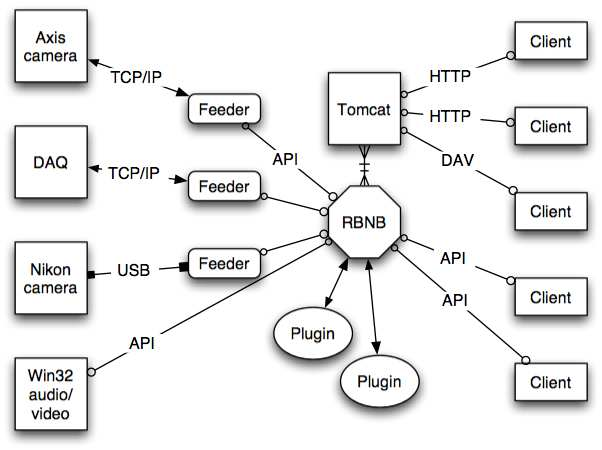
\includegraphics[scale=0.40]{figs/general-arch-diagram}} \quad
\subfigure[Typical architecture of a site with field deployed sensor system.\label{fig:fieldedsystem}]{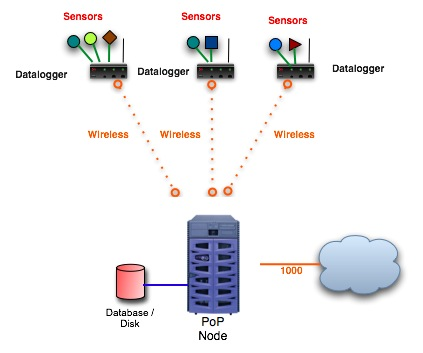
\includegraphics[scale=0.50]{figs/fieldedsystem}}
}
\caption{RBNB deployment and observing system}
\label{fig:rbnb-general-arch}
\end{center}
\end{figure*}    

We now briefly describe a typical sensor network setup for environmental and ecological monitoring applications (ref. figure~\ref{fig:fieldedsystem}). Typically, a digital or analog sensor is connected to a datalogger device, which acts as a simple computer to drive the sensor and store the results. The datalogger may be equipped with a wireless radio, allowing it to be periodically polled for data transfer. Some dataloggers are stand-alone, which means that a scientist must periodically visit the site to download data to a laptop or PDA. Davis, Campbell Scientific  Inc.~\cite{campbell}, National Instruments~\cite{ni} are examples of 
datalogger vendors. In fact, these common dataloggers encompass the majority of systems deployed by our collaborating domain scientists (ref. Section~\ref{sec:domains}). 


%  In the next section we give background information on RBNB DataTurbine and in Section~\ref{sec:rbnb-features} we describe how RBNB DataTurbine satisfies these requirements.

%

%Issues such as global warming, invasive species, infectious diseases,
%desertification, salination, pollution, and land use all present 
%difficult and challenging scientific questions. Rapid advancements in 
%the development and deployment of cyberinfrastructure and its wireless 
%extensions to sensor networks (embedded cyberinfrastructure) are playing 
%a key role in addressing these grand scientific challenges. To that end,
%existing and emerging large-scale observing systems comprising hundreds
%to thousands of sensors will gather data at the prescribed spatial
%and temporal granularity. NEON~\cite{NEON}, NEES~\cite{NEES}, GLEON~\cite{GLEON},
%CREON~\cite{CREON}, ORION~\cite{ORION}, and EarthScope~\cite{earthscope} are examples of 
%such large-scale observatories which would consist of thousands of sensors, 
%tens of thousands of data streams, and tens of thousands of end users. 
%These observing systems strive to take a comprehensive approach by gathering
%real-time multi-resolution observations, generating quality scientific products (e.g. models and 
%forecasts), and facilitating collaboration across scientists, programs, agencies, countries.
%These observing systems consist of a network of geographically distributed sites.
%We now describe two common observing system models.

%\begin{figure*}
%\begin{center}
%\mbox{
%\subfigure[Observing systems: federated model.\label{fig:obsdist}]{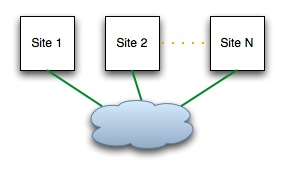
\includegraphics[scale=0.40]{figs/obsdist}} \quad
%\subfigure[Observing systems: centralized model.\label{fig:obs-center}]{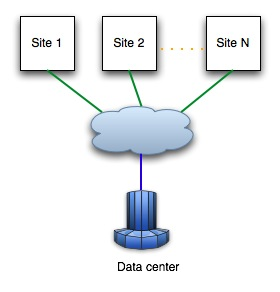
\includegraphics[scale=0.40]{figs/obs-center}}
%}
%\caption{Observing system models}
%\label{fig:obsmodel}
%\end{center}
%\end{figure*}    

%\emph{Federated model:} Participating sites are geographically distributed and are administrated locally (under autonomous control), at the site-level (ref. Figure~\ref{fig:obsdist}). In particular, each site can design its own architecture, database schema and manage its own data using that schema. Thus, the system from sensor to data resource, and the interfaces to the rest of the participating sites (and the world) are the responsibility of the site. 

%\emph{Centralized model:} Participating sites are geographically distributed but are administrated by a single administrative authority (ref. Figure~\ref{fig:obsdist}). All the sites gather their data and typically stream/upload it to a data center typically following a common database schema. It is therefore the responsibility of the data center to make the data available for the entire network of participants.

%This paper is based on our experience in providing cyberinfrastructure to a number of observing systems domains and communities.  %All of them face similar challenges in deploying and managing a distributed collection of heterogeneous sensors and instruments.  Few of them have the resources to buy and customize a commercial solution.  
%We briefly describe some representative domains here, and the interested reader is invited to pursue the references for more information.

%The National Ecological Observatory Network (NEON) will be the first national ecological measurement and observation system designed both to answer regional- to continental-scale scientific questions and to have the interdisciplinary participation necessary to achieve credible ecological forecasting and prediction~\cite{NEON}. A key requirement for NEON is robust streaming data middleware to handle thousands of data streams from a large variety of sensing devices. NEON is designed around the data center model.
%The Network for Earthquake Engineering and Simulation (NEES) is a shared national network of fifteen experimental facilities, collaborative tools, a centralized data repository~\cite{NEES}. NEES primarily follows the centralized model: post-experiment data is uploaded into a data center. However, it also has aspects of the federated model in that sites collaborating on distributed experiments use RBNB DataTurbine to stream data between laboratories. The Global Lake Ecological Observatory Network (GLEON) is a grassroots network of limnologists, information technology experts, and engineers who have a common goal of building a scalable, persistent network of lake ecology observatories~\cite{GLEON}.  GLEON follows the federated data model. The Coral Reef Environmental Observatory Network (CREON) is a worldwide collaborative association of scientists and engineers working to design marine sensor networks~\cite{CREON}. CREON also follows the federated data model.

%All these projects have similar CI requirements with regard to data acquisition, instrument management, and state-of-health monitoring including, reliable data capture and transport, persistent monitoring of numerous data channels, automated processing, event detection, analysis, integration across heterogeneous resources and systems, real-time tasking and remote operations and secure access to system resources. To that end, streaming data middleware provides the framework for application 
%development and integration. In the next section we give background information on RBNB DataTurbine
%and in Section~\ref{sec:rbnb-features} we describe how RBNB DataTurbine satisfies these requirements.